\begin{figure}[tb]

{\centering 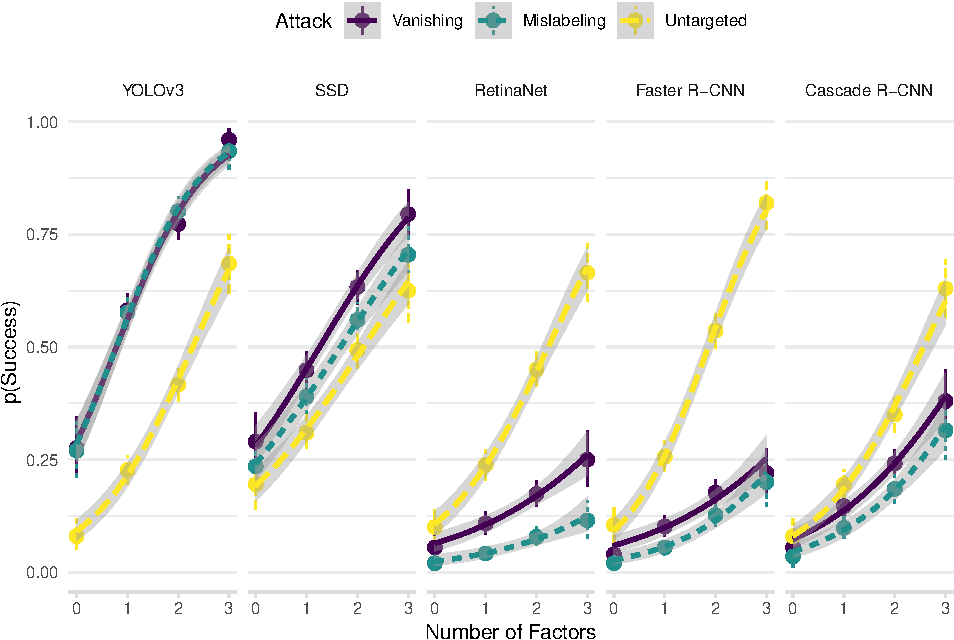
\includegraphics[width=1\linewidth]{imgs/biased_trend_graph} 

}

\caption{\textbf{Success factors can be exploited in combination to significantly increase success rates:}  We sampled target and perturb objects based on three validated success factors in Table \ref{tab:results_table} by targeting objects with low predicted confidence, perturbing large objects and selecting target and perturb objects close to one another. The binned summaries and regression trendlines graph success proportion against number of factors in the deliberate attack experiment. Errors are 95\% confidence intervals and every point aggregates success over 200 images. Success rates significantly increase as the number of factors combined increases. Significance is determined at $\alpha < 0.05$ using a Wald z-test on the logistic estimates. Full details are given in Section \ref{sec:del_per}.}\label{fig:biased_trend_graph}
\end{figure}